%%%%%%%%%%%%%%%%%%%%%%%%%%%%%%%%%%%%%%%%%
% Beamer Presentation
% LaTeX Template
% Version 1.0 (10/11/12)
%
% This template has been downloaded from:
% http://www.LaTeXTemplates.com
%
% License:
% CC BY-NC-SA 3.0 (http://creativecommons.org/licenses/by-nc-sa/3.0/)
%
%%%%%%%%%%%%%%%%%%%%%%%%%%%%%%%%%%%%%%%%%

%----------------------------------------------------------------------------------------
%	PACKAGES AND THEMES
%----------------------------------------------------------------------------------------

\documentclass{beamer}

\mode<presentation> {

% The Beamer class comes with a number of default slide themes
% which change the colors and layouts of slides. Below this is a list
% of all the themes, uncomment each in turn to see what they look like.

%\usetheme{default}
%\usetheme{AnnArbor}
%\usetheme{Antibes}
%\usetheme{Bergen}
%\usetheme{Berkeley}
%\usetheme{Berlin}
%\usetheme{Boadilla}
%\usetheme{CambridgeUS}
%\usetheme{Copenhagen}
%\usetheme{Darmstadt}
%\usetheme{Dresden}
%\usetheme{Frankfurt}
%\usetheme{Goettingen}
%\usetheme{Hannover}
%\usetheme{Ilmenau}
%\usetheme{JuanLesPins}
%\usetheme{Luebeck}
%\usetheme{Madrid}
%\usetheme{Malmoe}
%\usetheme{Marburg}
%\usetheme{Montpellier}
\usetheme{PaloAlto}
%\usetheme{Pittsburgh}
%\usetheme{Rochester}
%\usetheme{Singapore}
%\usetheme{Szeged}
%\usetheme{Warsaw}

% As well as themes, the Beamer class has a number of color themes
% for any slide theme. Uncomment each of these in turn to see how it
% changes the colors of your current slide theme.

%\usecolortheme{albatross}
%\usecolortheme{beaver}
%\usecolortheme{beetle}
%\usecolortheme{crane}
%\usecolortheme{dolphin}
%\usecolortheme{dove}
%\usecolortheme{fly}
%\usecolortheme{lily}
%\usecolortheme{orchid}
%\usecolortheme{rose}
%\usecolortheme{seagull}
\usecolortheme{seahorse}
%\usecolortheme{whale}
%\usecolortheme{wolverine}

\usefonttheme{structurebold}

\setbeamertemplate{footline} % To remove the footer line in all slides uncomment this line
%\setbeamertemplate{footline}[page number] % To replace the footer line in all slides with a simple slide count uncomment this line

\setbeamertemplate{navigation symbols}{} % To remove the navigation symbols from the bottom of all slides uncomment this line
}

\setbeamertemplate{items}[square]

\usepackage{graphicx} % Allows including images
\usepackage{booktabs} % Allows the use of \toprule, \midrule and \bottomrule in tables
\usepackage{textpos} % Package for text positioning
\usepackage{multimedia}


%----------------------------------------------------------------------------------------
%	TITLE PAGE
%----------------------------------------------------------------------------------------

\title[Microrod Lasing]{Toward Chip Integrated Ultra-Low-Noise Lasing Using a Microrod Resonator} % The short title appears at the bottom of every slide, the full title is only on the title page

\author[J. Becker]{Joe Becker \\
\scriptsize{W. Loh, F. Baynes, D. Cole, F. Quinlan, H. Lee,\\
K. Vahala, S. Papp, S. Diddams}} % Your name 

\titlegraphic{
\includegraphics[height=0.8cm]{Images/NIST_logo.png}}

\institute[NIST] % Your institution as it will appear on the bottom of every slide, may be shorthand to save space
{
National Institute of Standards and Technology\\ % Your institution for the title page
\medskip
\textit{Joe.Becker@nist.gov} % Your email address
}

\date{April 15, 2015} % Date, can be changed to a custom date

%\setbeamercolor{block title}{fg=black, bg=yellow}
%\setbeamercolor{title}{fg=black, bg=yellow}
%\setbeamercolor{frametitle}{fg=black, bg=yellow}
%\setbeamercolor{title in sidebar}{use=normal text,fg=black}
%\setbeamercolor{author in sidebar}{use=normal text,fg=black}
%\setbeamercolor{section in sidebar}{use=normal text,fg=black}
%\setbeamercolor{section in sidebar shaded}{use=normal text,fg=black!75!white}
%\setbeamercolor{item}{fg=black}

%titlepage logo
\addtobeamertemplate{frametitle}{}{%
\begin{textblock*}{3cm}(-2cm,-1cm)

\includegraphics[width=1.4cm,keepaspectratio]{Images/NIST_logo.png}
\end{textblock*}}


\begin{document}

\begin{frame}
\titlepage % Print the title page as the first slide
\end{frame}

\begin{frame}
\frametitle{Overview} % Table of contents slide, comment this block out to remove it
\tableofcontents % Throughout your presentation, if you choose to use \section{} and \subsection{} commands, these will automatically be printed on this slide as an overview of your presentation
\end{frame}


%%%%%%%%%PRESENTATION SLIDES%%%%%%%%

\section{Background} 
\begin{frame}\frametitle{Brillouin Lasers}
\begin{columns}
\column{0.5\textwidth}
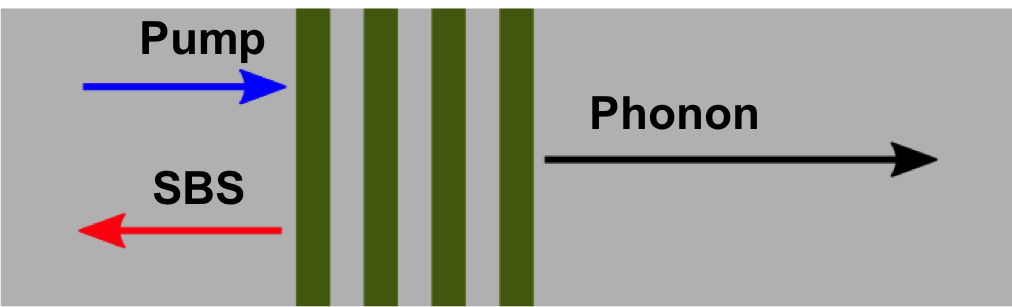
\includegraphics[width=5cm,keepaspectratio]{Images/SBS_Figure.png}

\column{0.5\textwidth}
\begin{block}{Gain Process}
\begin{itemize}
\item Pump scatters off of the phonons generating a stimulated Brillouin wave in the counter propagating direction 
\item SBS and pump fields interact to drive phonons to reinforce Brillouin wave generation
\end{itemize}
\end{block}

\end{columns}
\end{frame}

\begin{frame}\frametitle{Silica $\mu$rod Resonators}
\movie[width=3cm,height=2cm,poster]{}{Microrod_Fabrication.avi}

\end{frame}

\section{Motivations}
\begin{frame}\frametitle{Low Noise Laser Applications}
\end{frame}

\begin{frame}\frametitle{Current SBS Fiber Lasers}
\end{frame}


\section{Experiment}
\begin{frame}\frametitle{Apparatus}
\end{frame}

\section{Results}
\begin{frame}\frametitle{SBS Microrod Laser Frequency Noise}
\end{frame}

\begin{frame}\frametitle{SBS Microrod Laser Intensity Noise}
\end{frame}

\begin{frame}\frametitle{SBS Microrod Laser RF Spectrum}
\end{frame}

\section{Conclusions}
\begin{frame}\frametitle{Acknowledgments}
A special thanks to:

\begin{block}{My Advisors}
\begin{itemize}
\item Scott Diddams and Scott Papp
\end{itemize}
\end{block}

\begin{columns}
\column{0.5\textwidth}
\begin{block}{Optical Frequency Measurement Lab}
\begin{itemize}
\small
\item Fred Baynes
\item Katja Beha
\item Aur\'{e}lien Coillet
\item Daniel Cole
\item Pascal Del'Haye
\item Adam Green
\item William Loh
\item Frank Quinlan
\end{itemize}
\end{block}

\column{0.5\textwidth}
\begin{block}{The Caltech Vahala Group}
\begin{itemize}
\small
\item Hansuek Lee
\item Kerry Vahala
\end{itemize}
\end{block}

\begin{block}{Funding Provided By}
\small
The DARPA PULSE Program

\includegraphics[width=1.1\textwidth]{Images/DARPA_logo.png}
\end{block}

\end{columns}

\

\end{frame}

\begin{frame}\frametitle{Questions?}
\end{frame}



\end{document} 
